\chapter{Instability of Value Function Learning}
\label{chap:overestimation}

\begin{quote}
    This chapter is based on \longfullcite{hussing2024dissecting}.
\end{quote}

To improve sample efficiency, contemporary work in off-policy deep reinforcement learning (RL) has begun increasing the number of gradient updates per collected environment step~\parencite{janner2019mbpo,fedus2020revisiting,chen2021randomized, hiraoka2022dropout, nikishin2022primacy, doro2023barrier, schwarzer2023bigger, kim2023resetensemble}.  
However, as this update-to-data (UTD) ratio increases, value function learning seems to become unstable.
This is surprising, as neural networks have shown themselves to be generally robust to the number of update steps in other areas such as supervised classification.
In some cases, training for a very large number of steps actually increases the performance of neural networks, due to phenomena such as grokking \parencite{power2022grokking} or double descent \parencite{belkin2019reconciling}.
As such, this phenomenon should raise our suspicion that training \ac{drl} agents causes issues with neural networks that are not observed in other domains.

Notably, a recent study conjectured the emergence of a \emph{primacy bias} in deep actor critic algorithms, defined as ``a tendency to overfit initial experiences that damages the rest of the learning process''~\parencite{nikishin2022primacy}. 
This is a fairly broad explanation of the phenomenon, leaving room for investigation into \emph{how} fitting early experiences causes suboptimal learning behavior.

First approaches to tackle the learning failure challenges have been suggested, such as completely resetting networks periodically during the training process and then retraining them using the contents of the replay buffer~\parencite{nikishin2022primacy, doro2023barrier}. 
Resetting network parameters is a useful technique in that, in some sense, it can circumvent any ongoing optimization failures. 
Yet it seems likely that a more nuanced treatment of the various optimization challenges in deep RL might lead to more efficient training down the line, and provide more useful insights into how learning in 'ac{drl} evolves more generally. 
Especially for achieving efficient learning, throwing away all learned parameters and starting from scratch periodically is counter-productive, for instance in scenarios where, keeping all previous experience is infeasible. %
As such, we set out to study the components of early training that impair learning more closely and examine whether high-UTD learning without resetting is possible.


To motivate our study, we repeat the priming experiment of \textcite{nikishin2022primacy}, in which a network is updated for a large number of gradient steps on limited data. We show that during priming stages of training, value estimates diverge so far---and become so extreme---that it takes very long to unlearn them using new, counter-factual 
data. However, contrary to prior work, we find that it is not \emph{impossible} to learn even after priming, it merely takes a long time and many samples. 
This sparks hope for our endeavor of smooth learning in high-UTD regimes.
We show that compensating for the value function divergence allows learning to proceed. 
This suggests that the failure to learn does not stem from overfitting early data, which would result in correct value function on seen data, but rather from improperly fitting Q-values. 
We demonstrate that this divergence is most likely caused by prediction of out-of-distribution (OOD) actions that trigger large gradient updates, which destabilize feature learning.
Empirically, we find that instead of settling into fixed representations, the norm of the learned representations in the intermediate layers of the critic neural network grows.

The identified behavior, although triggered by OOD action prediction, seems to be more than the well-known overestimation due to statistical bias \parencite{thrun1993issues}. 
Instead, we hypothesize that the problem is an optimization failure and focus on mitigating the unbounded growth of the feature norm with architectural changes.
The main evidence for this hypothesis is that standard RL approaches to mitigating bias, such as minimization over two independent critic estimates~\parencite{fujimoto2018addressing}, are insufficient. 
In addition, using pessimistic updates~\parencite{fujimoto2019bcq, fujimoto2021td3bc} or regularization~\parencite{krogh1991simple, srivastava14dropout} to treat the value divergence can lead to suboptimal learning behavior, which is why architectural improvements are preferable in many cases.


We use a simple feature normalization method \parencite{zhang2019root, wang2020striving, bjorck2022is} that projects features onto the unit sphere.
This decouples learning the scale of the values from the first layers of the network and moves it to the last linear layer.
Empirically, this approach mitigates diverging Q-values in the priming experiment. 
Even after a large amount of priming steps, the agent immediately starts to learn. %
In a set of experiments on the \textsf{dm\_control} MuJoCo benchmarks~\parencite{tunyasuvunakool2020dmcontrol}, we show that accounting for value divergence can achieve significant across-task performance improvements when using high update ratios. 
Moreover, we achieve non-trivial performance on the challenging dog tasks that are often only tackled using model-based approaches. We demonstrate comparable performance with the recently developed TD-MPC2~\parencite{hansen2024tdmpc}, without using models or advanced policy search methods.


\section{Preliminaries} \label{sec:overestimation:preliminaries}

To fully elucidate the role that increasing the update ratio plays in destabilizing value function training, ostensibly necessitating resets, we present a series of small-scale experiments.

\section{Investigating the effects of large update-to-data ratios during priming} \label{sec:overestimation:investigating}

\begin{figure}[t!]
\centering
    \begin{subfigure}[b]{0.8\textwidth}
        \centering
        
\includegraphics[height=0.4cm]{figures/dissecting/priming/priming_base_return_legend.pdf}
    \end{subfigure}\\%
    \begin{subfigure}[b]{0.25\textwidth}
        \centering
        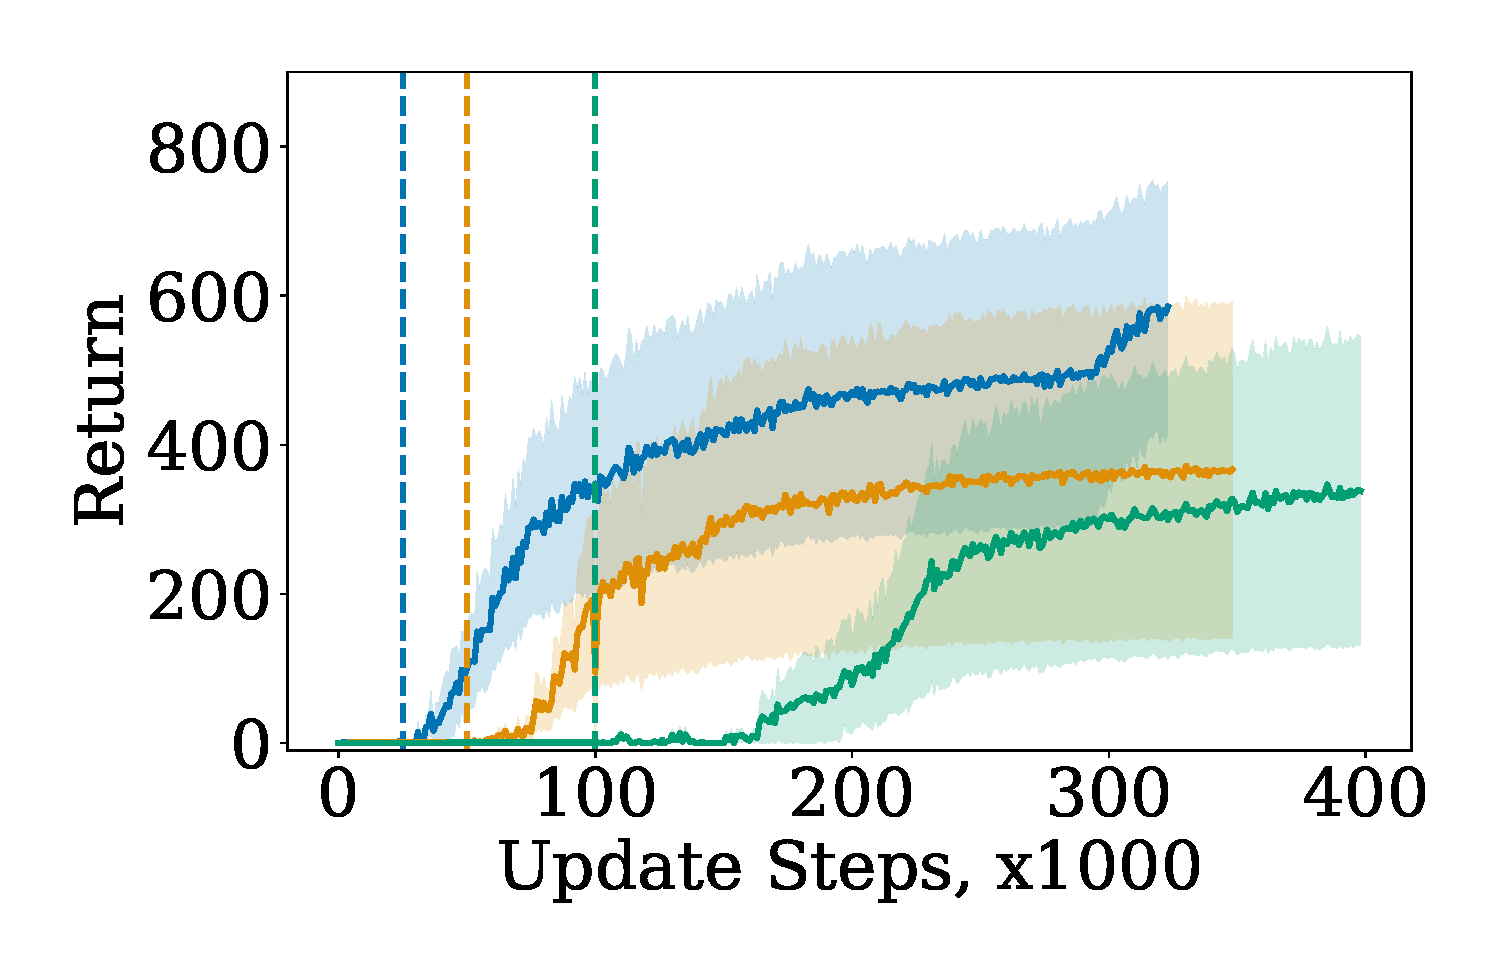
\includegraphics[width=3.7cm, trim=1cm 1cm 1cm 1cm ,clip]{figures/dissecting/priming/priming_base_return.pdf}
        \label{subfig:overestimation:overestimation:priming_base_ret}
    \end{subfigure}%
    \begin{subfigure}[b]{0.25\textwidth}
    \centering
        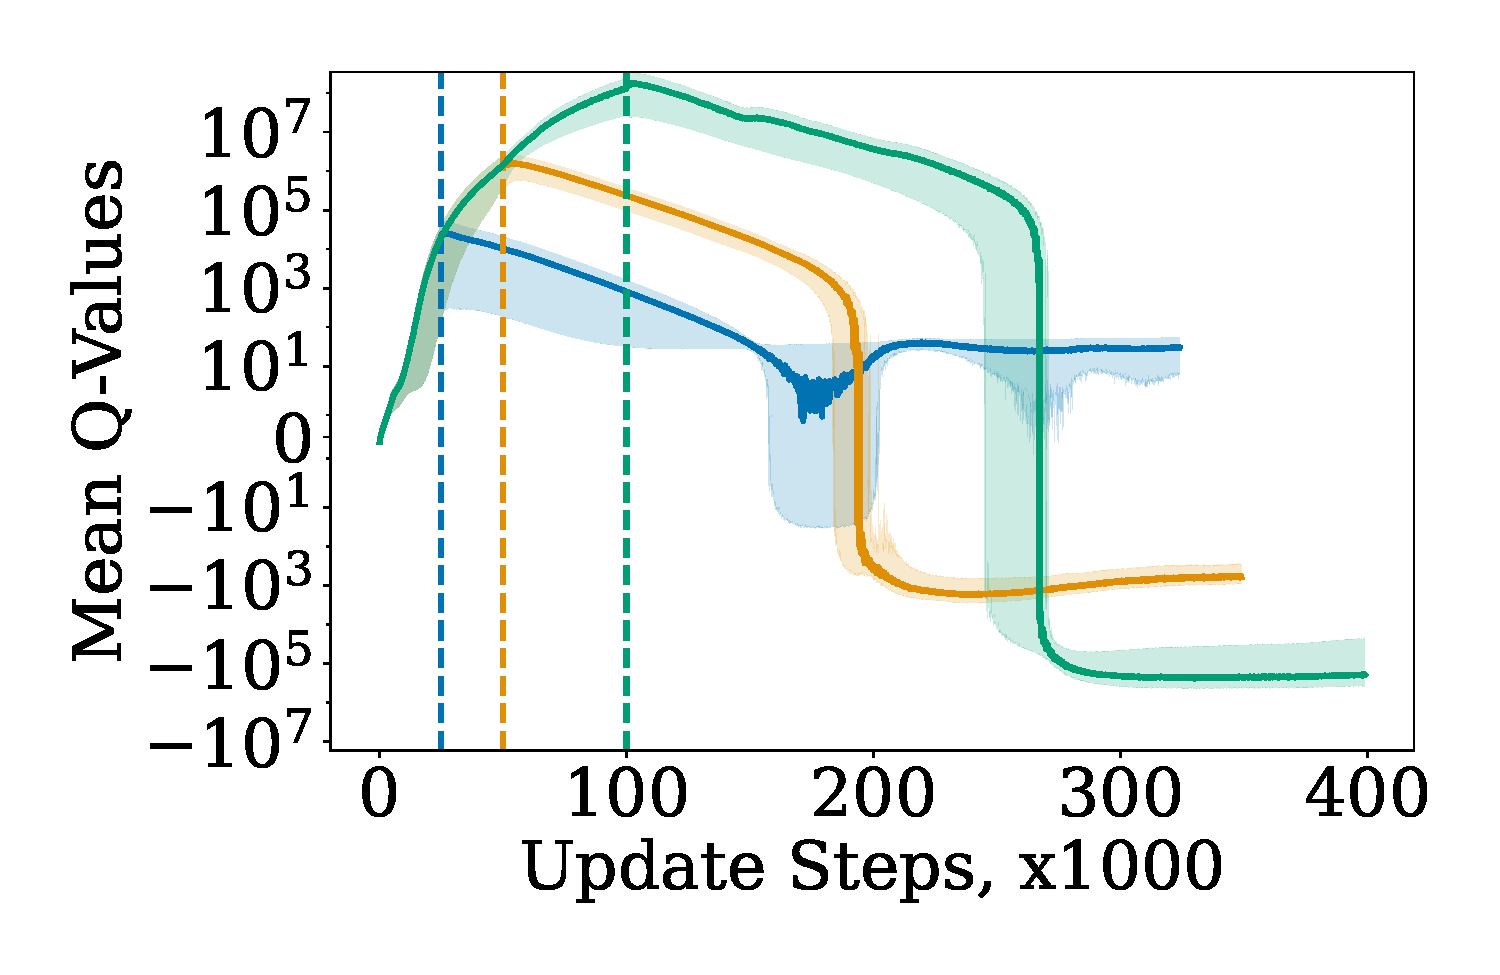
\includegraphics[width=3.7cm, trim=1cm 1cm 1cm 1cm ,clip]{figures/dissecting/priming/priming_base_Q.pdf}
        \label{subfig:overestimation:overestimation:priming_base_Q}
    \end{subfigure}%
    \begin{subfigure}[b]{0.25\textwidth}
        \centering
        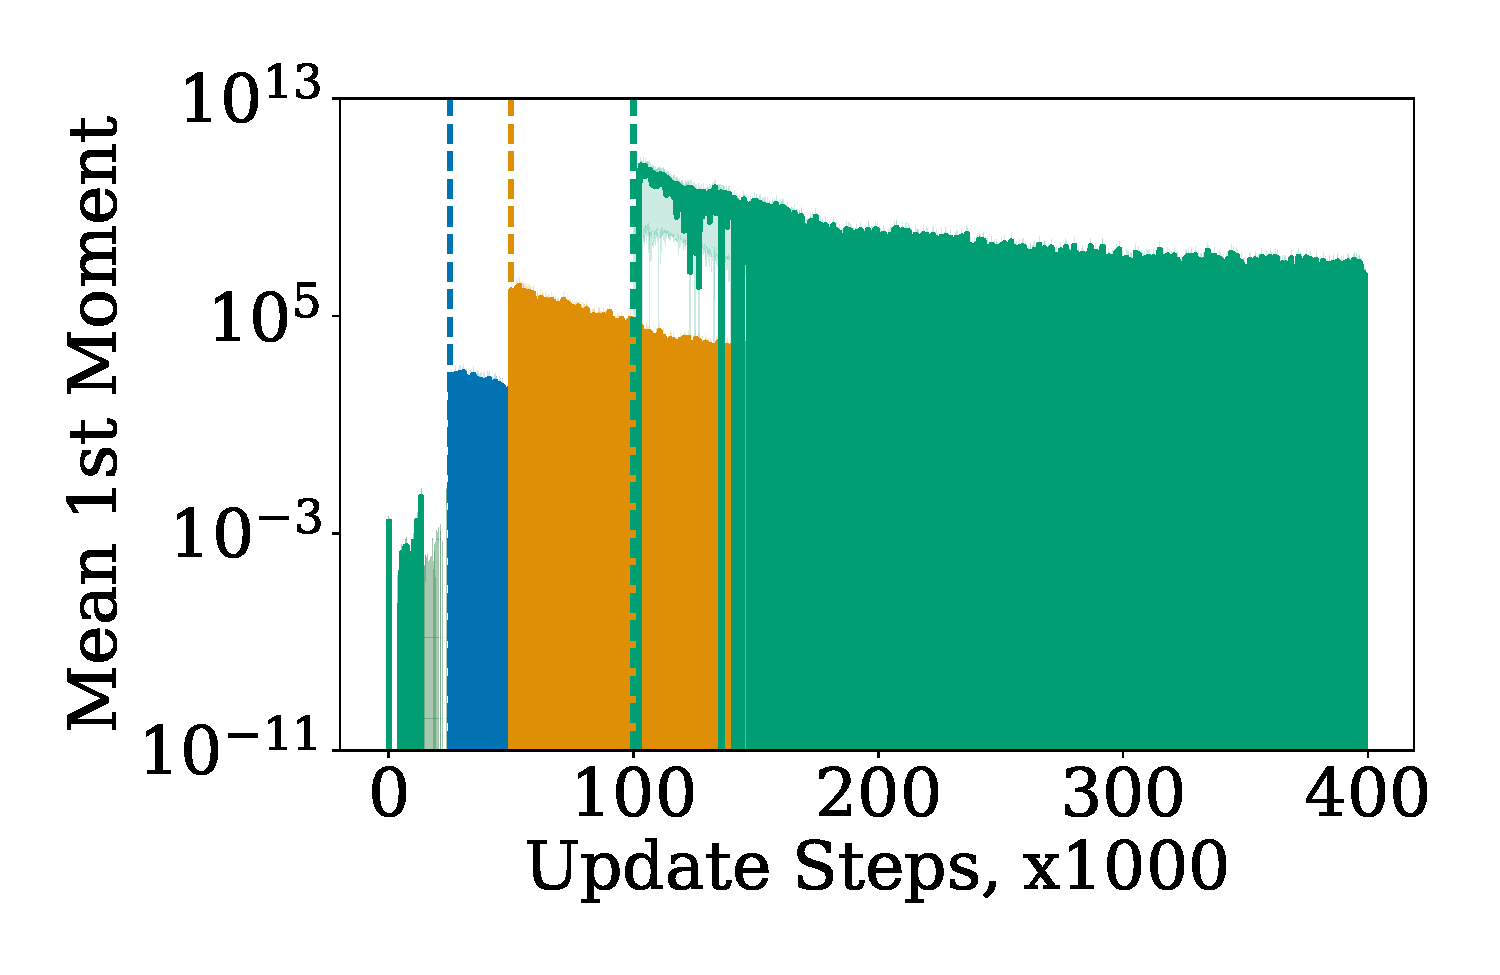
\includegraphics[width=3.7cm, trim=1cm 1cm 1cm 1cm ,clip]{figures/dissecting/priming/priming_base_exp_avg.pdf}
    \end{subfigure}%
    \begin{subfigure}[b]{0.25\textwidth}
        \centering
        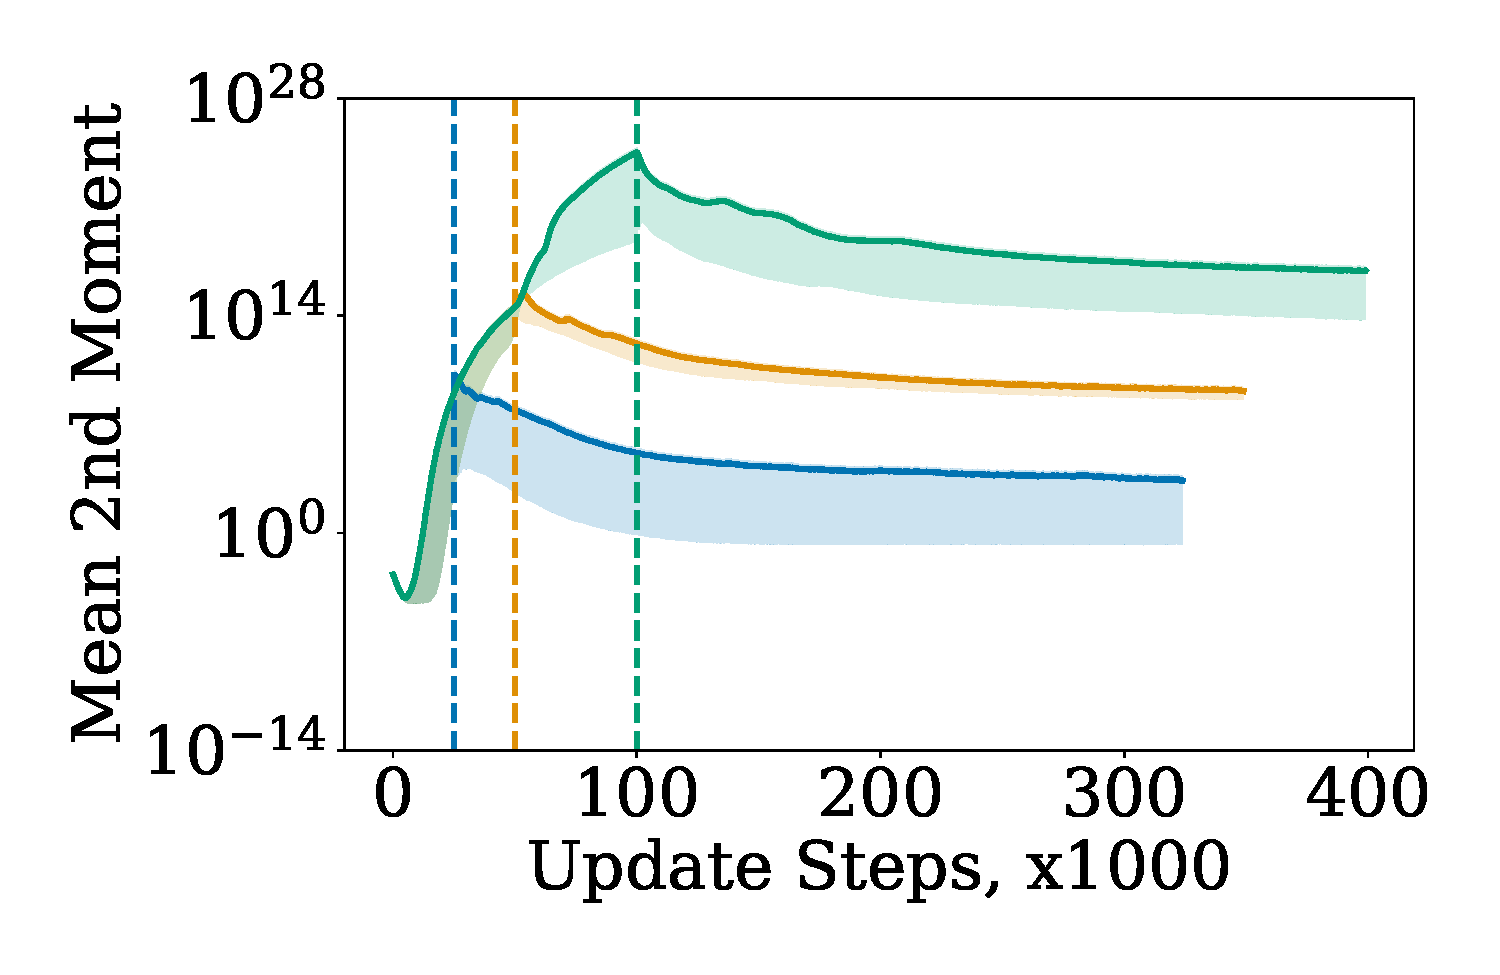
\includegraphics[width=3.7cm, trim=1cm 1cm 1cm 1cm ,clip]{figures/dissecting/priming/priming_base_exp_avg_sq.pdf}
    \end{subfigure}%
    \caption{Return, in-distribution Q-values and Adam optimizer moments during priming for different lengths. Dotted lines correspond to end of priming. More priming leads to lower return and larger Q-value and optimizer divergence.}
    \label{fig:overestimationpriming_base}
\end{figure}

As mentioned, the definition of the primacy bias is broad.
To obtain a more nuanced understanding, we set out to re-investigate the early stages of high-UTD training. To do so, we repeat the priming experiment conducted by~\textcite{nikishin2022primacy}.\footnote{For consistency with later sections, we use the ReLU activation here which can lead to unstable learning of other components. We repeat all the experiments with ELUs in Appendix~\ref{app:priming} to provide even stronger support of our findings.}
We first collect a small amount of random samples. Then, using the SAC algorithm, we perform a priming step, training the agent for a large number of updates without additional data. After priming, training continues as usual. Prior results reported by~\textcite{nikishin2022primacy} suggest that once the priming step has happened, agents lose their ability to learn completely. We use the simple Finger-spin task \parencite{tunyasuvunakool2020dmcontrol} to study the root causes for this systematic failure and to examine if there are ways to recover without resets. In this section, we report means over five random seeds with standard error in shaded regions. Hyperparameters are kept consistent with previous work for ease of comparison.

\subsection{An old acquaintance: Q-value overestimation} \label{sec:overestimation}
We first ask whether there is a barrier as to how many steps an agent can be primed for before it becomes unable to learn. We test this by collecting 1,000 samples and varying the number of updates during priming from 25,000 to 50,000 and 100,000. The results are presented in Figure~\ref{fig:overestimationpriming_base}. 

We make two key observations. First, lower amounts of priming are correlated with higher early performance. More precisely, it seems that many runs simply take longer before they start learning as the number of priming steps increases. Second, during priming the scale of the average Q-value estimates on observed state-action pairs increases drastically. We find that the Q-values start out at a reasonable level, but as priming goes on they eventually start to diverge drastically. Once the agent estimates very large Q-values, the final performance in terms of average returns deteriorates. We also observe that the second moment of the Adam optimizer~\parencite{kingma2015adam} is correlated with the divergence effect. Optimizer divergence has been observed before as a cause of plasticity loss under non-stationary data \parencite{lyle2023understanding}, but in our experiments the data is stationary during priming. We conjecture that the momentum terms lead to much quicker propagation of poor Q-values and ultimately to prediction of incorrect Q-values, even on in-distribution data.


After priming, there exist two cases: 1) either the Q-values need to be unlearned before the agent can make progress or 2) there is a large drop from very high to very low Q-values that is strongly correlated with loss in effective dimension of the embedding, as defined by~\cite{yang2020harnessing} (see Appendix~\ref{app:priming_dim}). In the second case, we find that contrary to previous claims in the literature, rank can sometimes be recovered upon seeing new, counter-factual data and the network continues to learn. Yet, in other cases the agent gets stuck at low effective dimension; a possible explanation for the failure to learn observed in the priming experiments of~\textcite{nikishin2022primacy}. This is orthogonal to a previously studied phenomenon where target network-based updates lead to perpetually reduced effective rank~\parencite{kumar2021implicit}.



\subsection{On the potential causes of divergence} \label{sec:causes}

\begin{figure}[t]
\begin{minipage}[b]{.35\textwidth}
\centering
    \begin{subfigure}[b]{\textwidth}
        \centering
        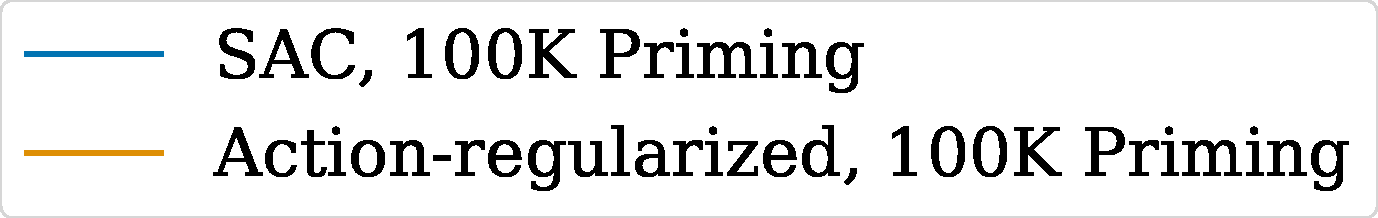
\includegraphics[height=0.8cm]{figures/dissecting/priming/priming_causes_return_legend.pdf}
    \end{subfigure}\\%
    \begin{subfigure}[b]{\textwidth}
        \centering
        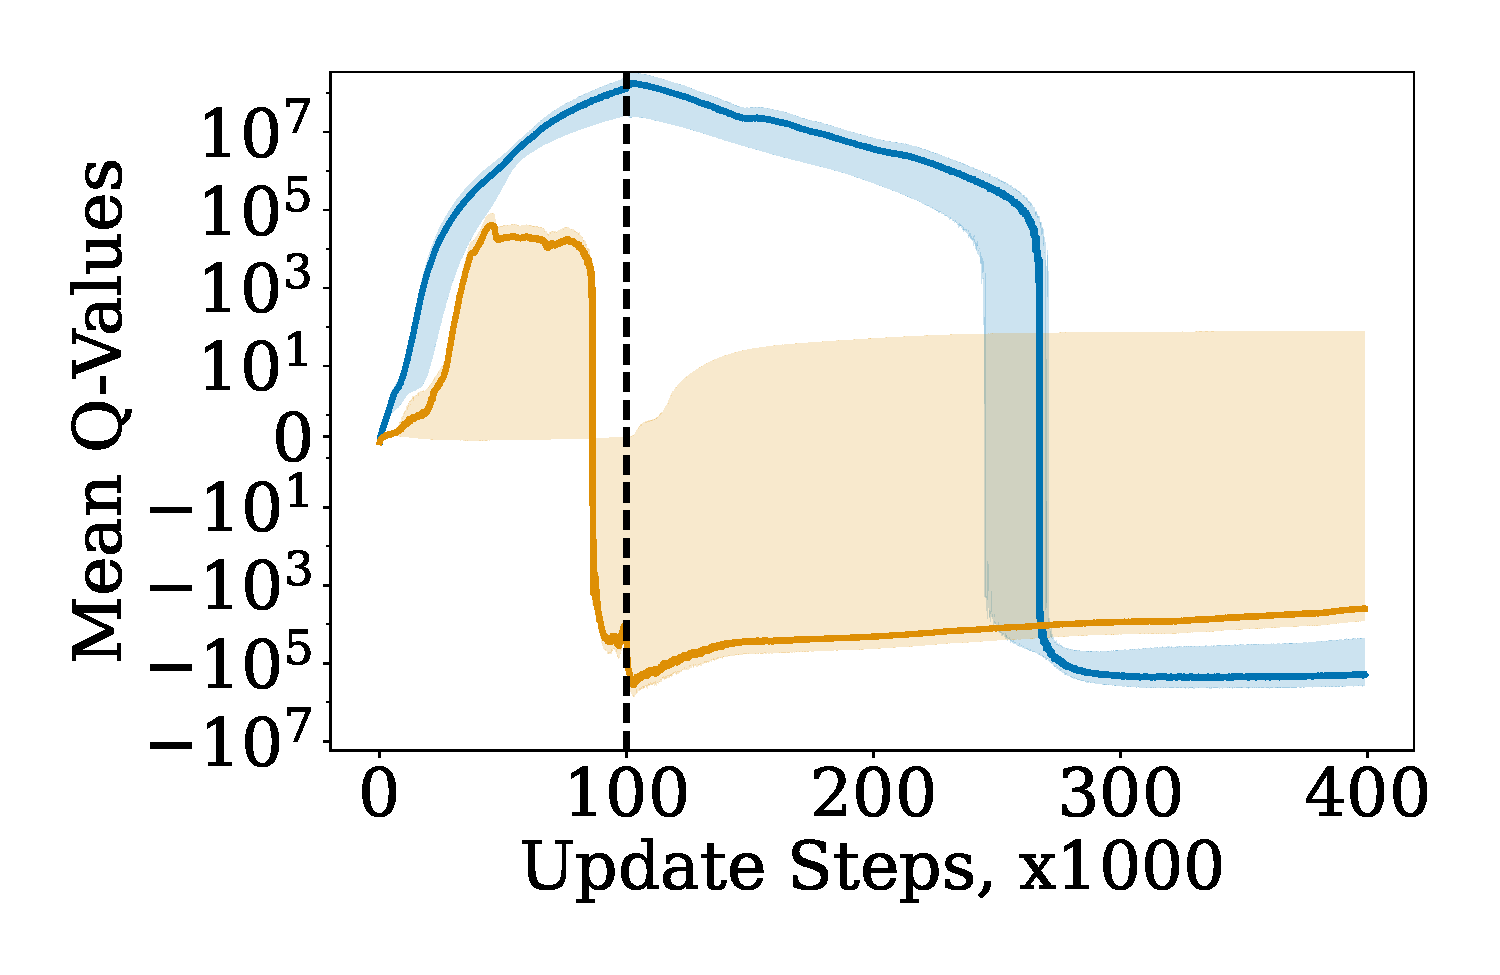
\includegraphics[width=4.8cm, trim=1cm 1cm 1cm 1cm ,clip]{figures/dissecting/priming/priming_causes_Q.pdf}
        \label{subfig:overestimation:priming_causes_Q}
    \end{subfigure}%
    \caption{Priming with SAC and action regularization during priming. The latter lowers divergence. }
    \label{fig:overestimationpriming_causes}
\end{minipage}
\hfill
\begin{minipage}[b]{.62\textwidth}
    \centering
    \begin{subfigure}[b]{0.8\textwidth}
        \centering
        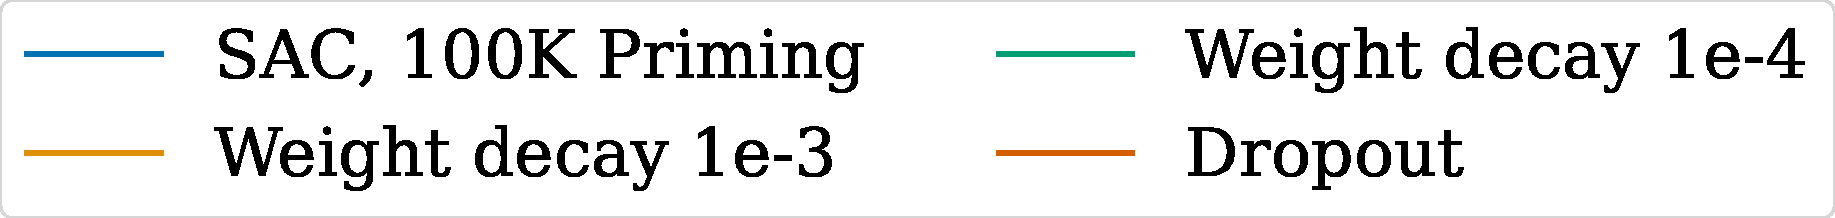
\includegraphics[height=0.8cm]{figures/dissecting/priming/priming_ablations_return_legend.pdf}
    \end{subfigure}\\%
    \begin{subfigure}[b]{0.5\textwidth}
        \centering
        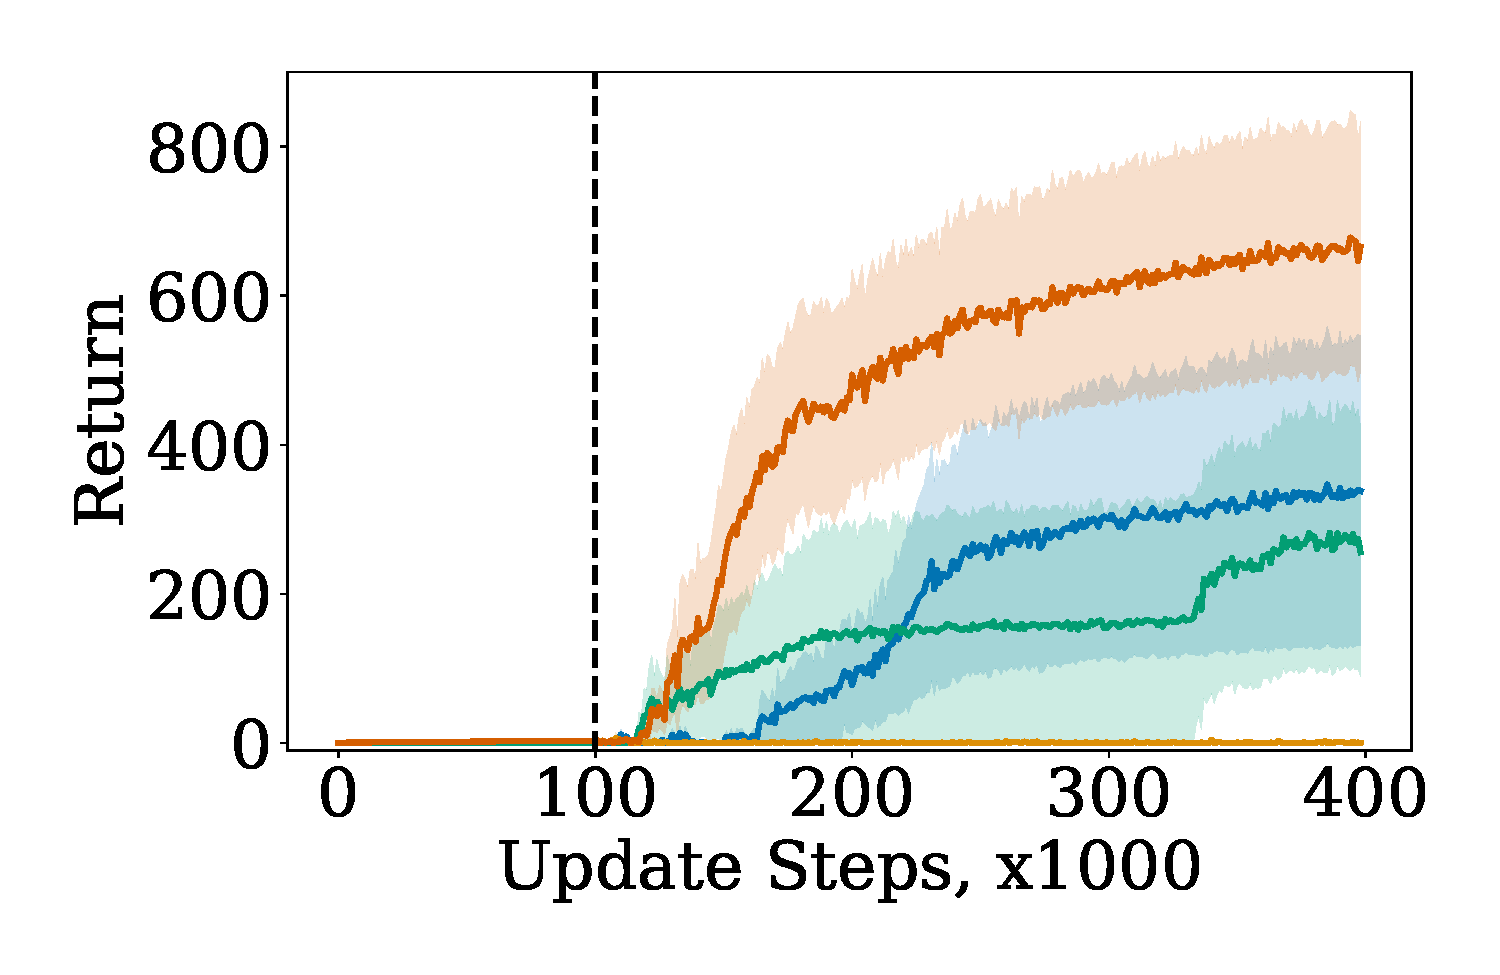
\includegraphics[width=4.8cm, trim=1cm 1cm 1cm 1cm ,clip]{figures/dissecting/priming/priming_ablations_return.pdf}
        \label{subfig:overestimation:priming_abl_ret}
    \end{subfigure}%
    \begin{subfigure}[b]{0.5\textwidth}
    \centering
        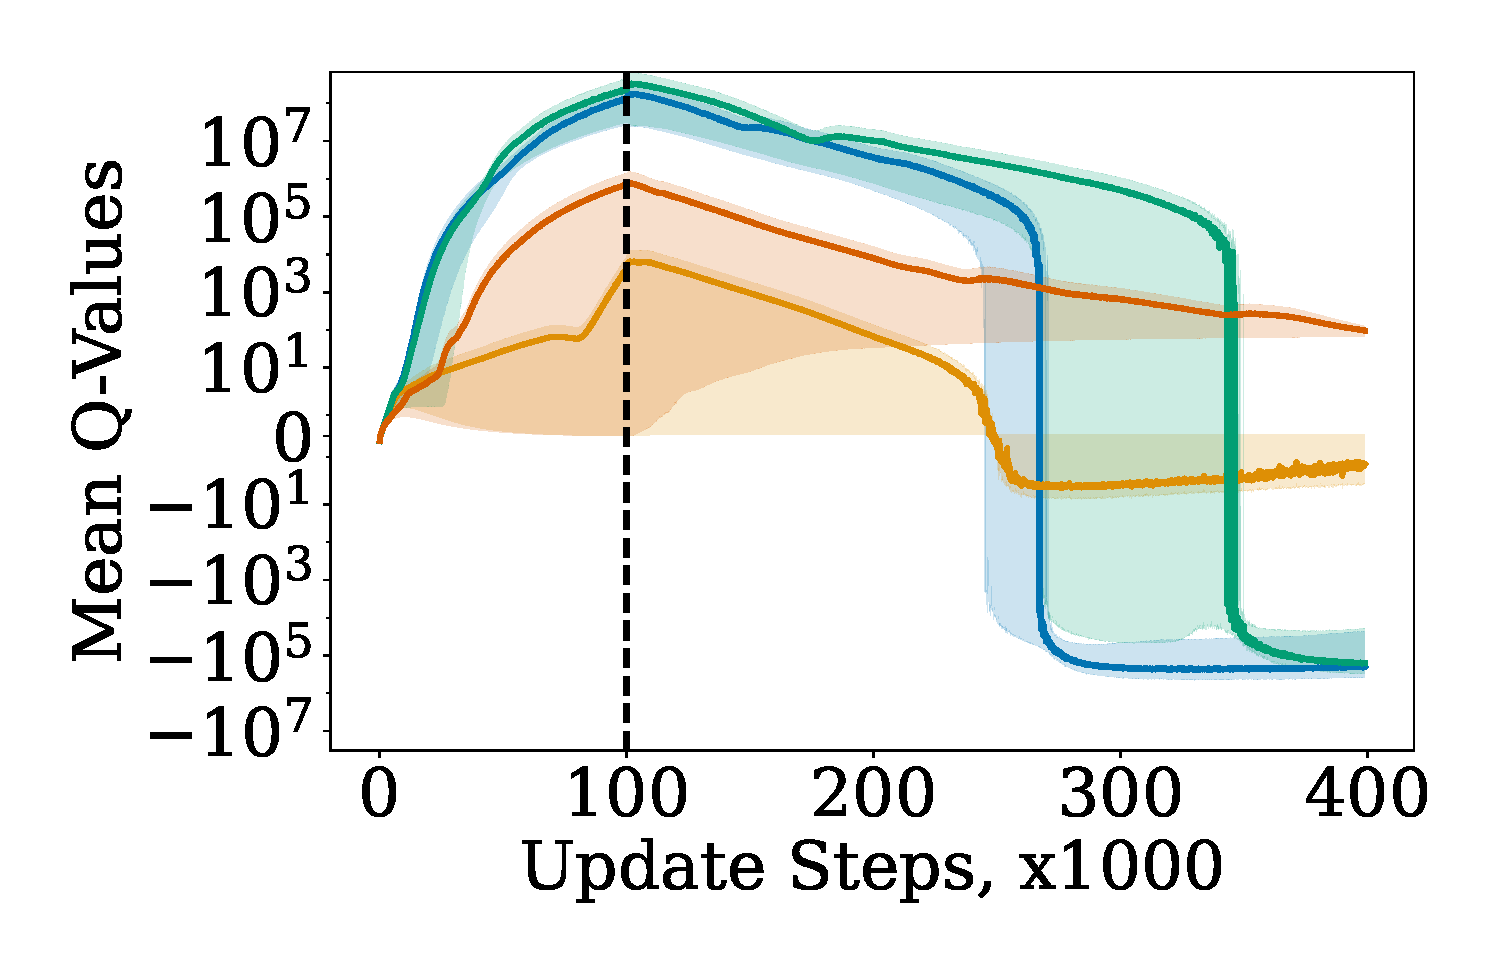
\includegraphics[width=4.8cm, trim=1cm 1cm 1cm 1cm ,clip]{figures/dissecting/priming/priming_ablations_Q.pdf}
        \label{subfig:overestimation:priming_abl_Q}
    \end{subfigure}%
    \caption{Return and
    Q-values of priming runs with weight decay and dropout. Results indicate that both regularizers mitigate priming to some extent but not sufficiently. }
    \label{fig:overestimationpriming_abl}
\end{minipage}
\end{figure}


We conjecture that Q-value divergence starts with overestimated values of OOD actions. This overestimation could cause the optimizer to continually increase Q-values via its momentum leading to divergence. 
To test this hypothesis, we add a conservative behavioral cloning~\parencite{pomerleau1988alvinn, atkeson1997robot} loss term to our actor that forces the policy to be close to replay buffer actions. Prior work employed this technique in offline RL to mitigate value overestimation~\parencite{fujimoto2021td3bc}. More formally, our actor update is extended by the loss $
        \mathcal{L}_{c, \psi} = \min_{\psi} \mathbb{E}_{a \sim \mathcal{D}, \hat{a} \sim \pi_{\psi}(\state)}[||a - \hat{a}||_2]$. 
The results in Figure~\ref{fig:overestimationpriming_causes} indicate that the basis of the conjecture is corroborated as divergence is much smaller---but not mitigated completely---when values are learned on actions similar to seen ones. However, in practice we do not know when divergence sets in, which limits the applicability of this technique in realistic scenarios. Using it throughout all of training, rather than just during priming, impairs the learner's ability to explore. We investigate the effects of the optimizer in more detail and provide preliminary evidence that the second-order term may be at fault in Appendix~\ref{app:priming_opt}. 




\subsection{Applying common regularization techniques} \label{sec:regularization}

Regularization is a common way to mitigate gradient explosion and is  often used to address overestimation~\parencite{farebrother2018generalization, chen2021randomized, liu2021regularization, hiraoka2022dropout, li2023efficient}. We investigate the priming experiments under techniques such as using L$^2$ weight decay~\parencite{krogh1991simple} or adding dropout~\parencite{srivastava14dropout} to our networks in Figure~\ref{fig:overestimationpriming_abl}.

Both L$^2$ weight decay as well as dropout can somewhat reduce the divergence during priming, however not to a sufficient degree.
While L$^2$ regularization fails to attain very high performance, dropout is able to recover a good amount of final return.
However, both methods require tuning of a hyperparameter that trades off the regularization term with the main loss.
This hyperparameter is environment-dependent and tuning it becomes infeasible for large UTD-ratios due to computational resource limitations. 
Still, the results imply that it is in fact possible to overcome the divergence in priming and continue to learn good policies.





\subsection{Divergence in practice} 
\label{sec:real}



One question that remains is whether we can find these divergence effects outside of the priming setup. We find that, while priming is an artificially constructed worst case, similar phenomena happen in regular training on standard benchmarks when increasing update ratios (see Figure~\ref{fig:overestimationhumanoid_failure}). Further, the divergence is not limited to early stages of training as it happens at arbitrary points in time.
We therefore conjecture that divergence is not a function of 
\begin{wrapfigure}{r}{0.54\textwidth}
  \begin{minipage}{\linewidth}
    \centering\captionsetup[subfigure]{justification=centering}
    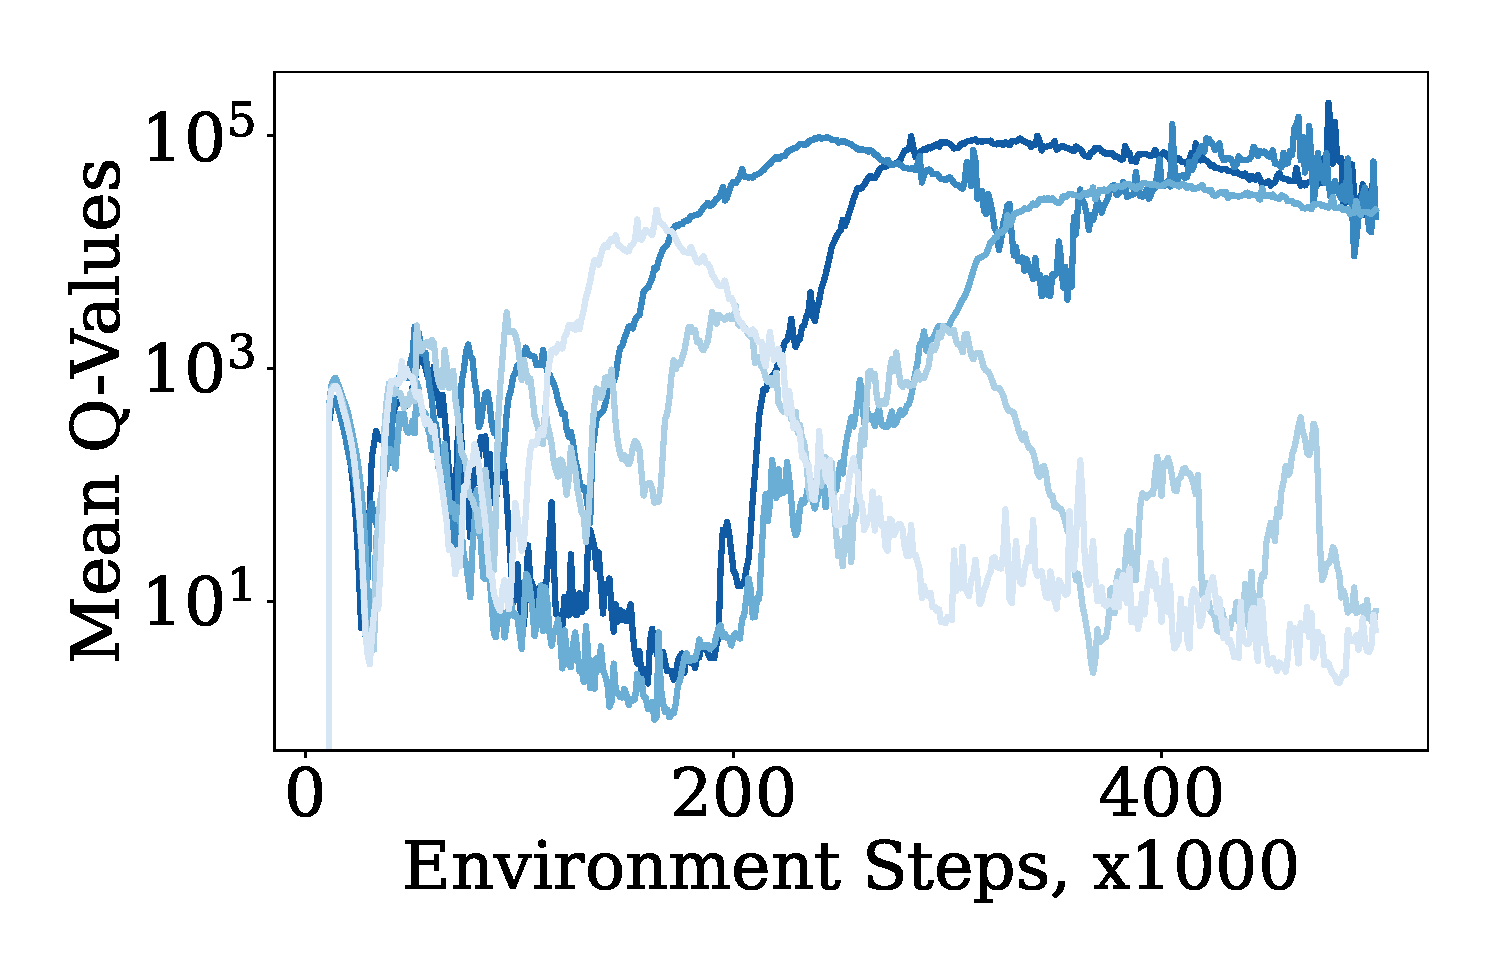
\includegraphics[width=4cm, trim=1cm 1cm 1cm 1cm ,clip]{figures/dissecting/priming/humanoid_Q.pdf}
    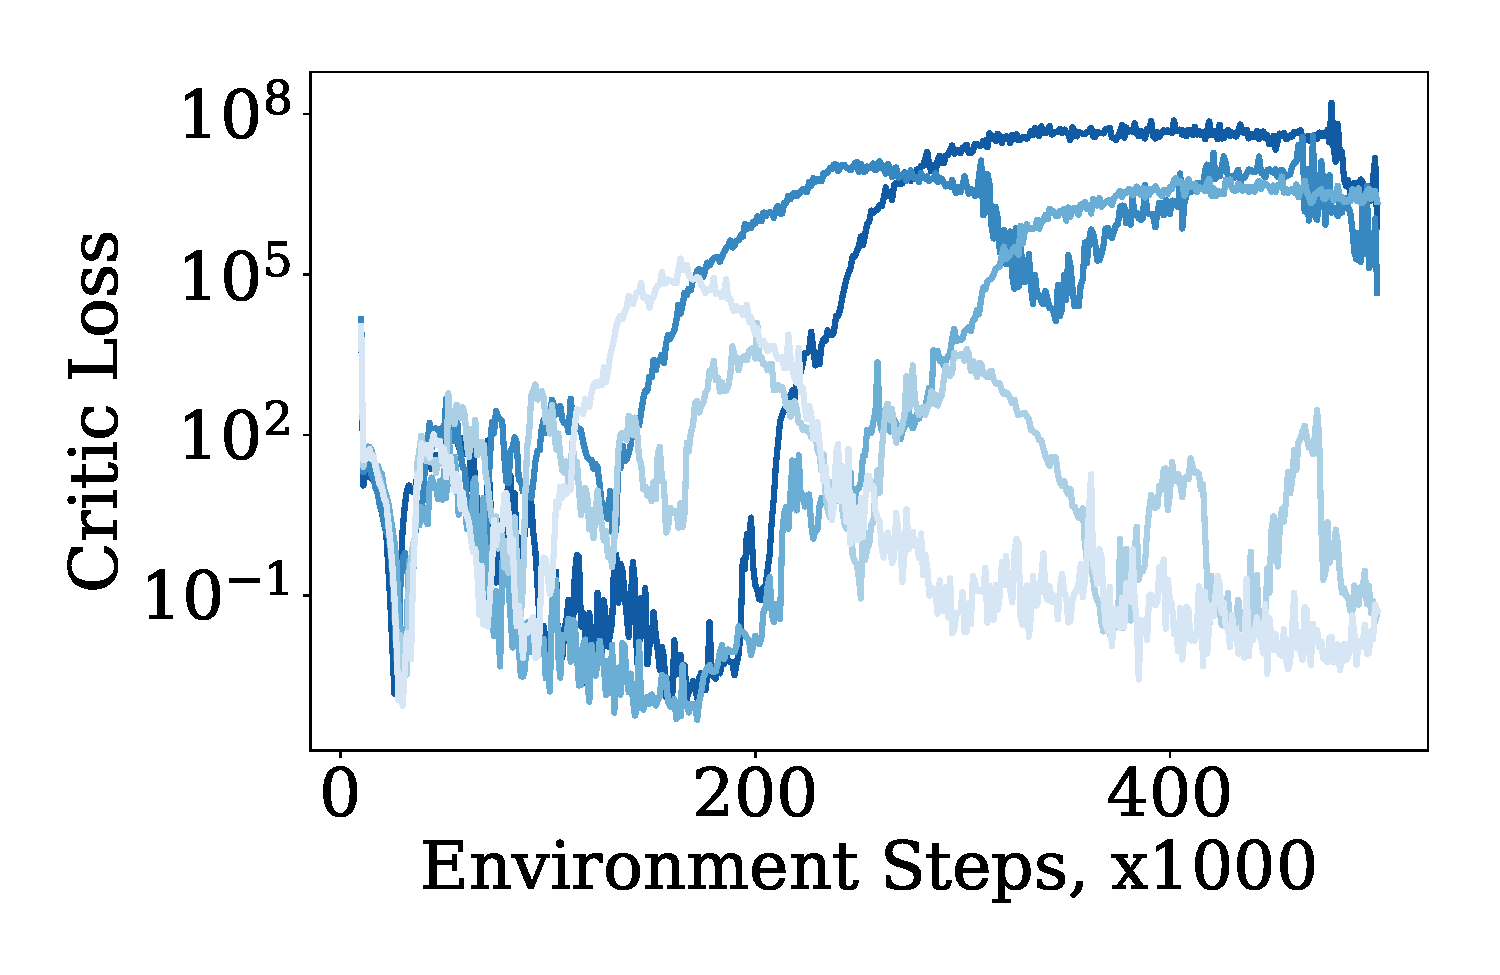
\includegraphics[width=4cm, trim=1cm 1cm 1cm 1cm ,clip]{figures/dissecting/priming/humanoid_loss.pdf}
    \caption{In-distribution Q-values and critic loss of five SAC seeds on the humanoid-run task using $\mathrm{UTD}=32$. Values diverge at arbitrary time-points, not only during the beginning. Loss mirrors Q-value divergence.}
    \label{fig:overestimationhumanoid_failure}
  \end{minipage}
\end{wrapfigure}
amount of experience but rather one of state-action space coverage. Note that the reported Q-values have been measured on the observed training data, not on any out-of-distribution state-action pairs. 
The respective critic losses become very large. All this points toward a failure to fit Q-values. This behavior does not align with our common understanding of overfitting~\parencite{bishop2006pattern},  challenging the hypothesis that high-UTD learning fails merely due to large validation error~\parencite{li2023efficient}.

\section{Towards high-UTD optimization without resetting} \label{sec:method}

Regularization techniques such as those in Section~\ref{sec:regularization} can fail to alleviate divergence as they tend to operate across the whole network and lower the weights everywhere even if higher values are actually indicated by the data. They also require costly hyperparameter tuning. Thus, we turn towards network architecture changes to the commonly used MLPs that have proven useful in overcoming issues such as exploding gradients in other domains~\parencite{ba2016layer, xu2019understanding}. 

\subsection{Limiting gradient explosion via unit ball normalization} \label{sec:unitball}

\begin{figure}[t]
\begin{minipage}[t]{.60\textwidth}
\centering
    \begin{subfigure}[b]{\textwidth}
        \centering
        
\includegraphics[height=0.4cm]{figures/dissecting/priming/priming_norm_return_legend.pdf}
    \end{subfigure}\\%
    \begin{subfigure}[b]{0.5\textwidth}
        \centering
        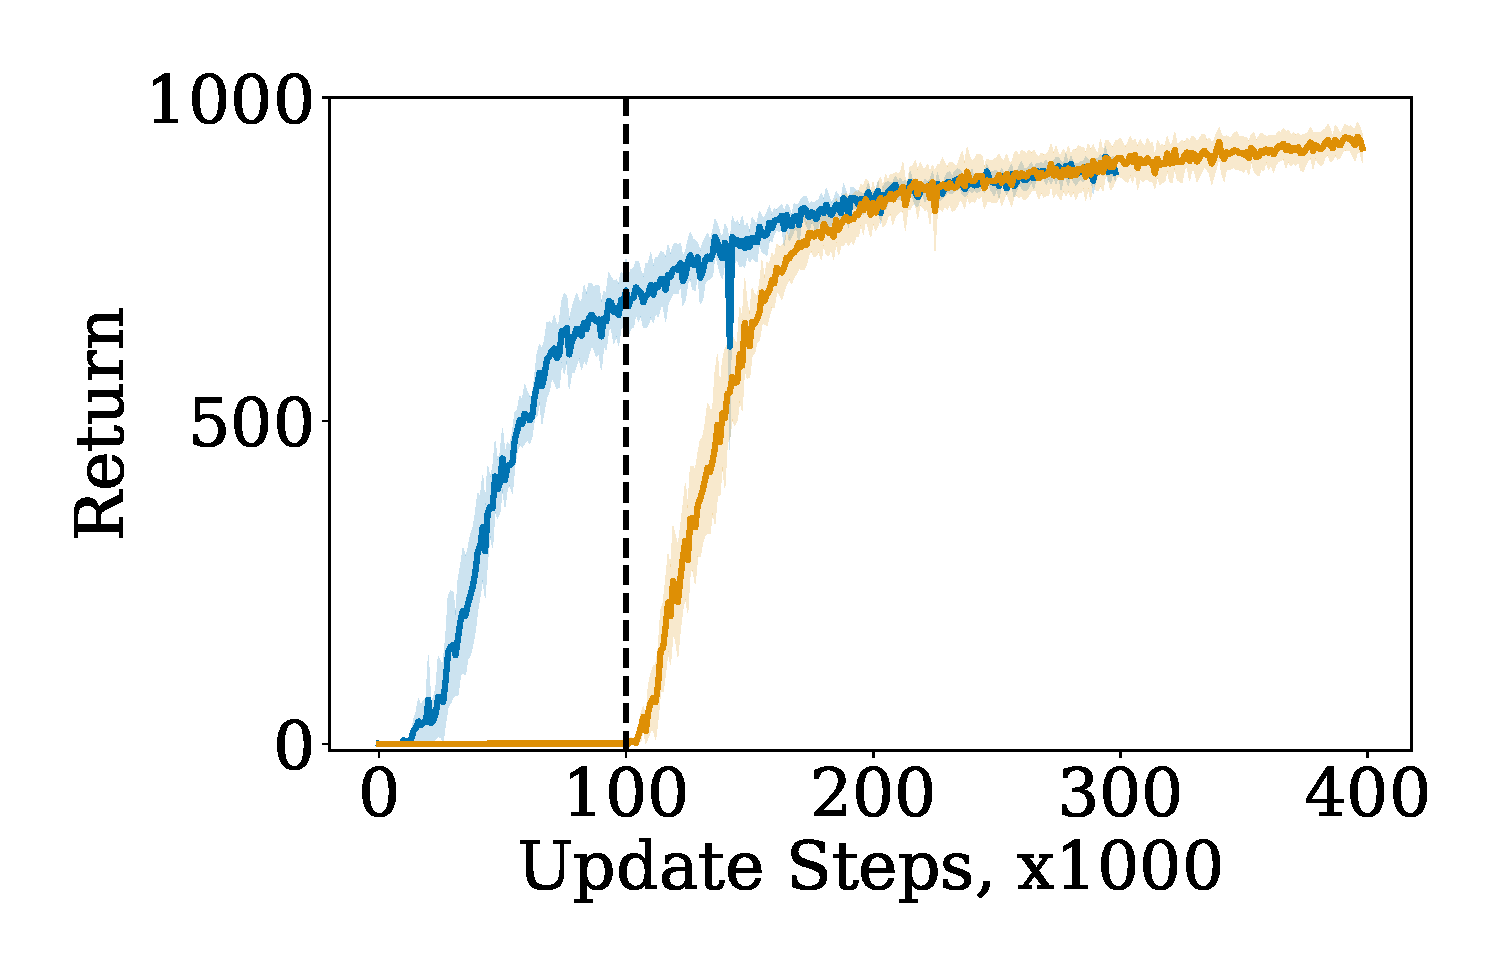
\includegraphics[width=4.8cm]{figures/dissecting/priming/priming_norm_return.pdf}
        \label{subfig:overestimation:priming_norm_ret}
    \end{subfigure}%
    \begin{subfigure}[b]{0.5\textwidth}
        \centering
        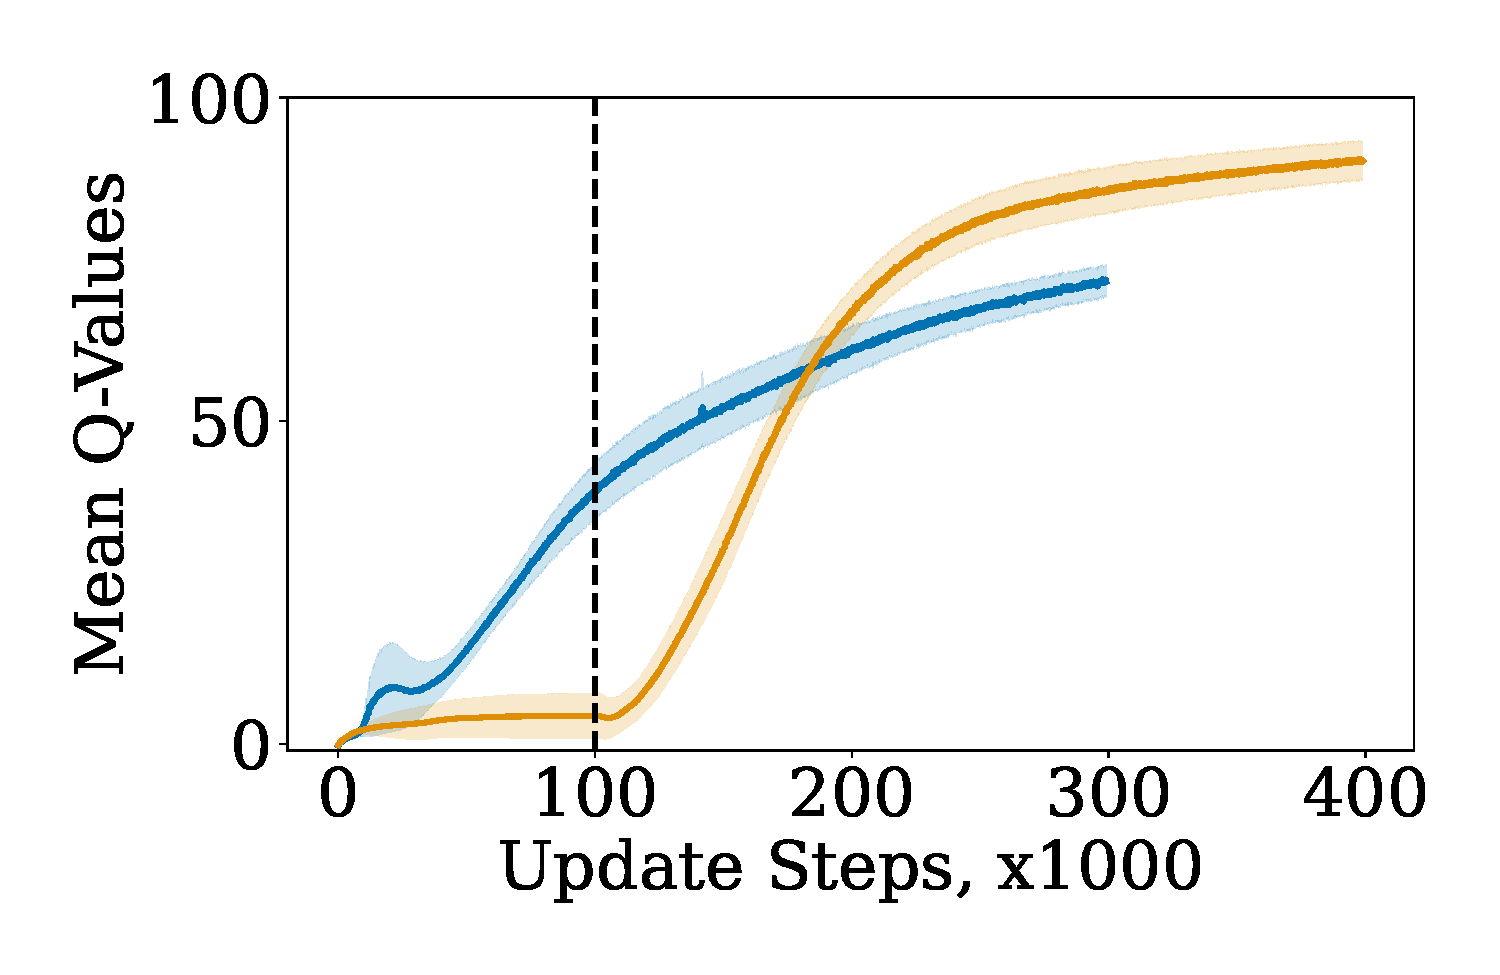
\includegraphics[width=4.8cm]{figures/dissecting/priming/priming_norm_Q.pdf}
        \label{subfig:overestimation:priming_norm_Q}
    \end{subfigure}%
    \caption{(Left) Return and (Right) Q-values comparing SGD result and OFN when priming for 100K steps. OFN obtains returns close to that of the well-trained SGD agent and learns an appropriate Q-value scale correctly.}
    \label{fig:overestimationpriming_norm}
\end{minipage}
\hfill
\begin{minipage}[t]{.36\textwidth}
\centering
    \begin{subfigure}[b]{\textwidth}
        \centering
        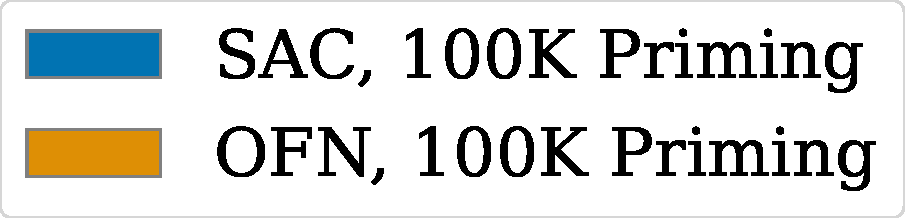
\includegraphics[height=0.8cm]{figures/dissecting/priming/weight_magnitudes_legend.pdf}
    \end{subfigure}
    \\%
    \begin{subfigure}[b]{\textwidth}
        \centering
        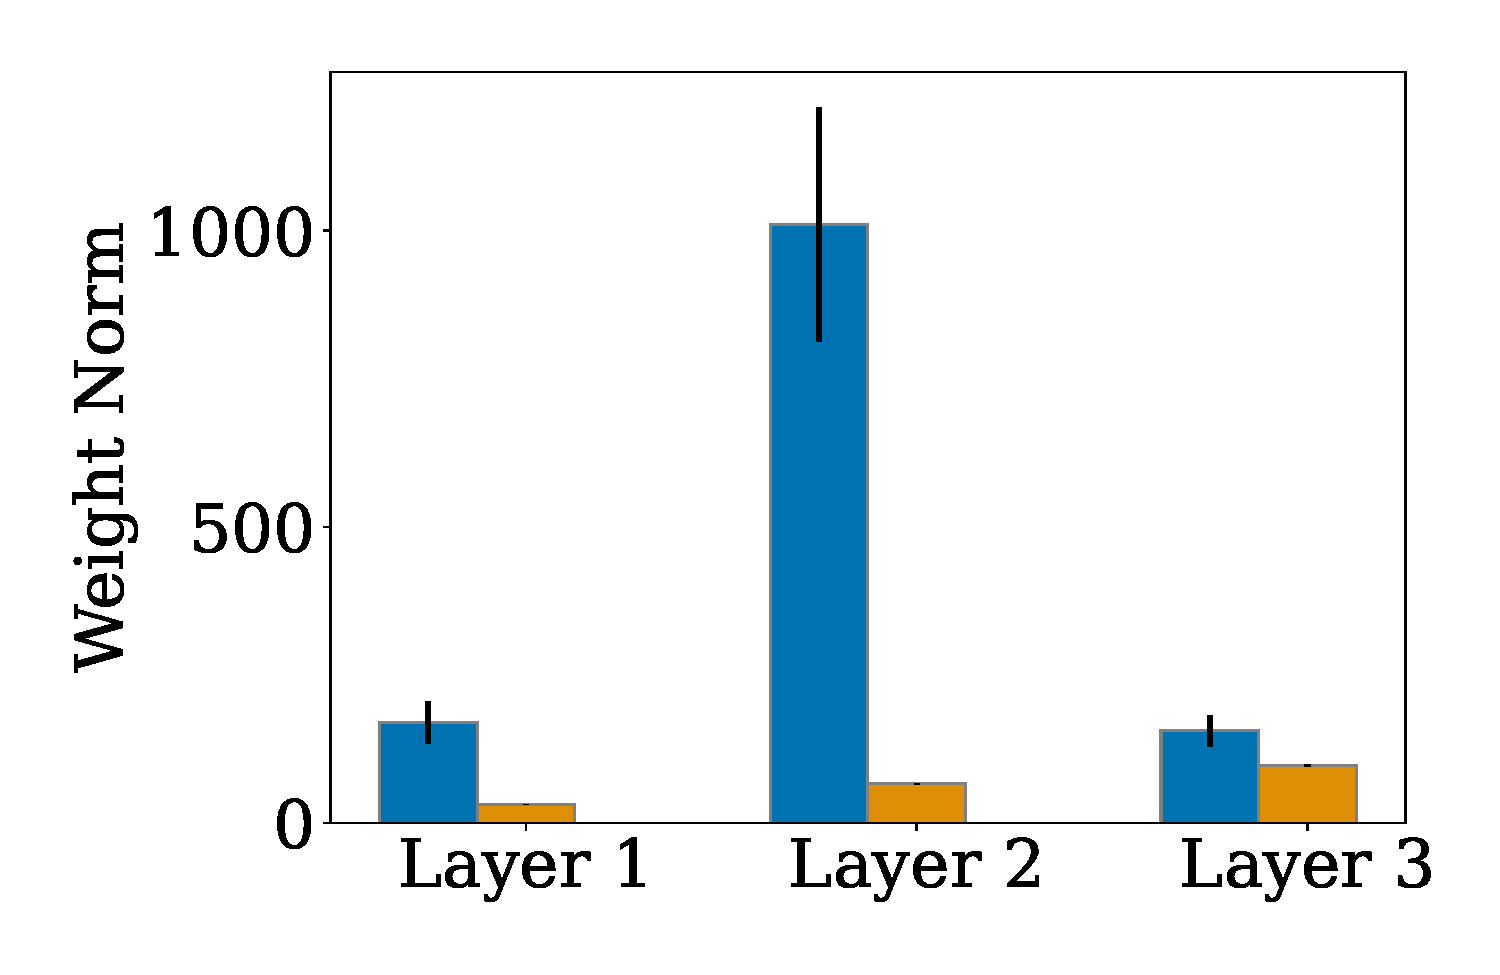
\includegraphics[width=4.6cm]{figures/dissecting/priming/weight_magnitudes.pdf}
    \end{subfigure}%
    \caption{$L_2$ norm of network weights per layer after priming for default and OFN  architectures. OFN leads to smaller weights and significant mass in the last layer.}
    \label{fig:overestimationweight_norm}
\end{minipage}
\end{figure}

As discussed previously, the prediction of an unknown action might trigger the propagation of a large, harmful gradient. Further, the Q-values of our network ought to grow over time as they more closely approximate those of a good policy. If we predict incorrectly on one of these Q-values, a potentially very large loss is propagated. Gradients are magnified by multiplicative backpropagation via ReLU activations~\parencite{glorot2011deep} as well as momentum from Adam~\parencite{kingma2015adam}. Note that all resulting issues arise in the early network layers. 
We hypothesize that we can address many of these problems by separating the scaling of the Q-values to the appropriate size from the earlier non-linear layers of the network and moving the Q-value scaling to the final linear layer.

One contender to achieve the value decoupling described in the previous paragraph is layer normalization~\parencite{ba2016layer}, but one would have to disable scaling factors used in common implementations. Still, standard layer normalization would not guarantee small features everywhere. Instead, we use a stronger constraint and project the output features of the critic encoder onto the unit ball using the function
$f(\mathbf{x}) = \frac{\mathbf{x} }{\|\mathbf{x}\|_2}$~\parencite{zhang2019root}, 
where $\|\cdot\|_2$ denotes the L$^2$ vector norm and $\mathbf{x}$ is the output of our encoder $\phi(\state, a)$. This ensures that all values are strictly between $0$ and $1$ and the gradients will be tangent to the unit sphere. Note that this function's gradient is not necessarily bounded to ensure low gradient propagation (see Appendix~\ref{app:unitnorm}), but we argue that if large values are never created in the early layers, gradient explosion will not occur. The unit ball has previously been used to mitigate large action prediction in the actor~\parencite{wang2020striving} or to stabilize RL training in general~\parencite{bjorck2022is}. 
For brevity, we will refer to this method as {\em output feature normalization} (OFN). We solely apply OFN to the critic, unlike~\textcite{wang2020striving}, since our goal is to mitigate value divergence. OFN is very simple and requires only a one-line change in implementation.

\subsection{Evaluating feature output normalization during priming} \label{sec:evalmethod}

To test the efficacy of the OFN-based approach, we repeat the priming experiment in Figure~\ref{fig:overestimationpriming_norm}.
We find that OFN achieves high reward and most distinctly, Q-value divergence during priming is fully mitigated. 
Note also that we are using a discount factor of $\gamma = 0.99$, returns are collected over 1,000 timesteps and rewards are in $[0, 1]$. 
We therefore expect the average Q-values to be roughly at $10\%$ of the undiscounted return which seems correct for the OFN network. 
However, more importantly, as shown in Figure~\ref{fig:overestimationweight_norm}, most of the Q-value scaling happens in the last layer.

\section{Experimental evaluation}

We evaluate our findings on the commonly used \textsf{dm\_control} suite~\parencite{tunyasuvunakool2020dmcontrol}. All results are averaged over ten random seeds.\footnote{For comparison with TD-MPC2~\parencite{hansen2024tdmpc} we use data provided by their implementation, which only contains three seeds. As the goal is not to rank algorithmic performance but to give intuition about the relative strengths of adapting the network architecture, we believe that this is sufficient in this case.} We report evaluation returns similar to~\textcite{nikishin2022primacy}, which we record every 10,000 environment steps. We compare a standard two-layer MLP with ReLU ~\parencite{nair2010rectified} activations, both with and without resetting, to the same MLP with OFN. %
The architecture is standard in many reference implementations. Architecture and the resetting protocol are taken from \textcite{doro2023barrier} and hyperparameters are kept without new tuning to ensure comparability of the results. More details can be found in Appendix~\ref{app:impl}.

To understand the efficacy of output normalization on real environments under high UTD ratios, we set out to answer multiple questions that will illuminate RL optimization failures:\\
{\bf Q1:}~Can we maintain learning without resetting neural networks?\\
{\bf Q2:}~Are there other failure modes beside Q-value divergence under high UTD ratios?\\
{\bf Q3:}~When resets alone fall short, can architectural changes enable better high-UTD training?

\subsection{Feature normalization stabilizes high-UTD training} 

\begin{figure}[t]
\begin{minipage}[b]{0.67\textwidth}
\centering
    \begin{subfigure}[b]{\textwidth}
        \centering
        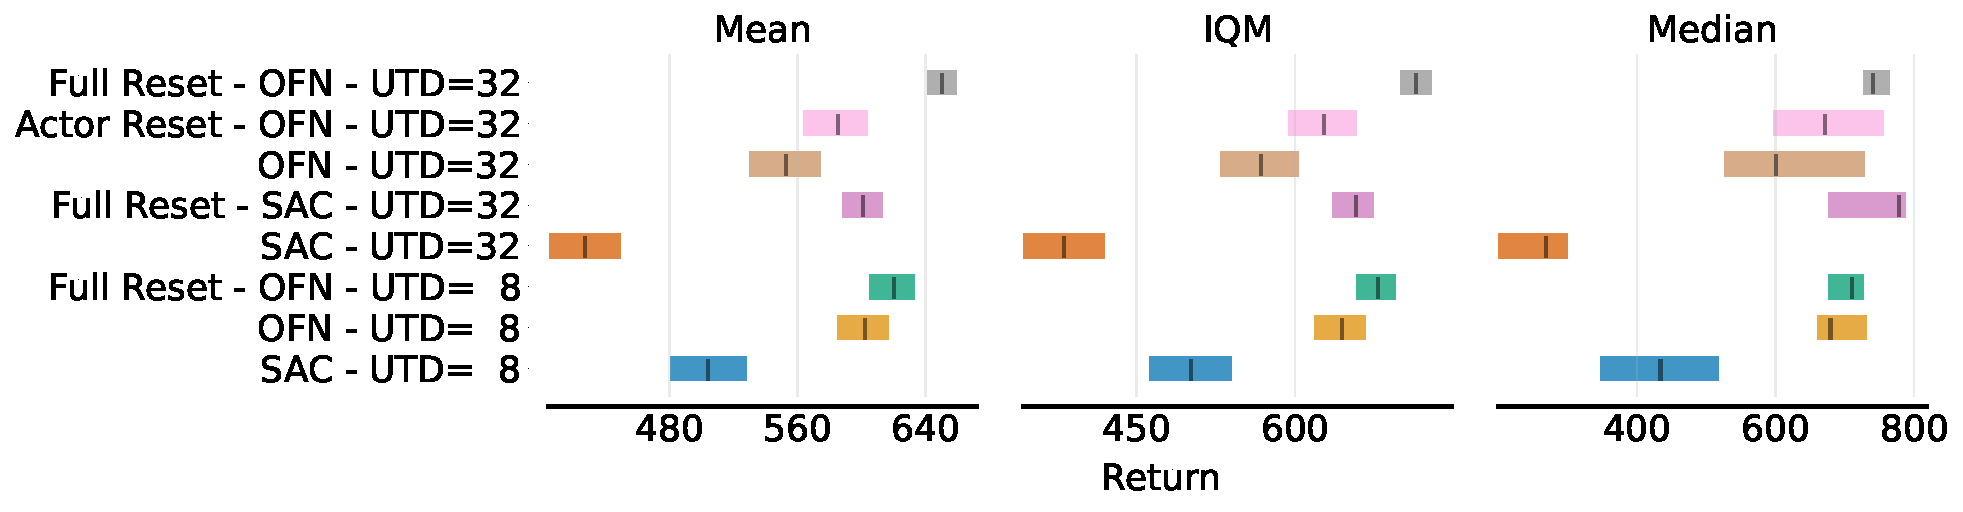
\includegraphics[width=10.2cm]{figures/dissecting/main_exp/all_aggregate_scores.pdf}
    \end{subfigure}%
    \caption{Mean, interquartile mean (IQM), and median with $95\%$ bootstrapped confidence intervals of standard SAC and OFN on the DMC15-500k Suite. OFN can maintain high performance even under large UTD. OFN with $\mathrm{UTD} = 8$ achieves comparable performance to standard resetting with $\mathrm{UTD} = 32$ across metrics.}
    \label{fig:overestimationaggregate}
\end{minipage}
\hfill
\begin{minipage}[b]{.3\textwidth}
\centering
    \begin{subfigure}[b]{\textwidth}
        \centering
        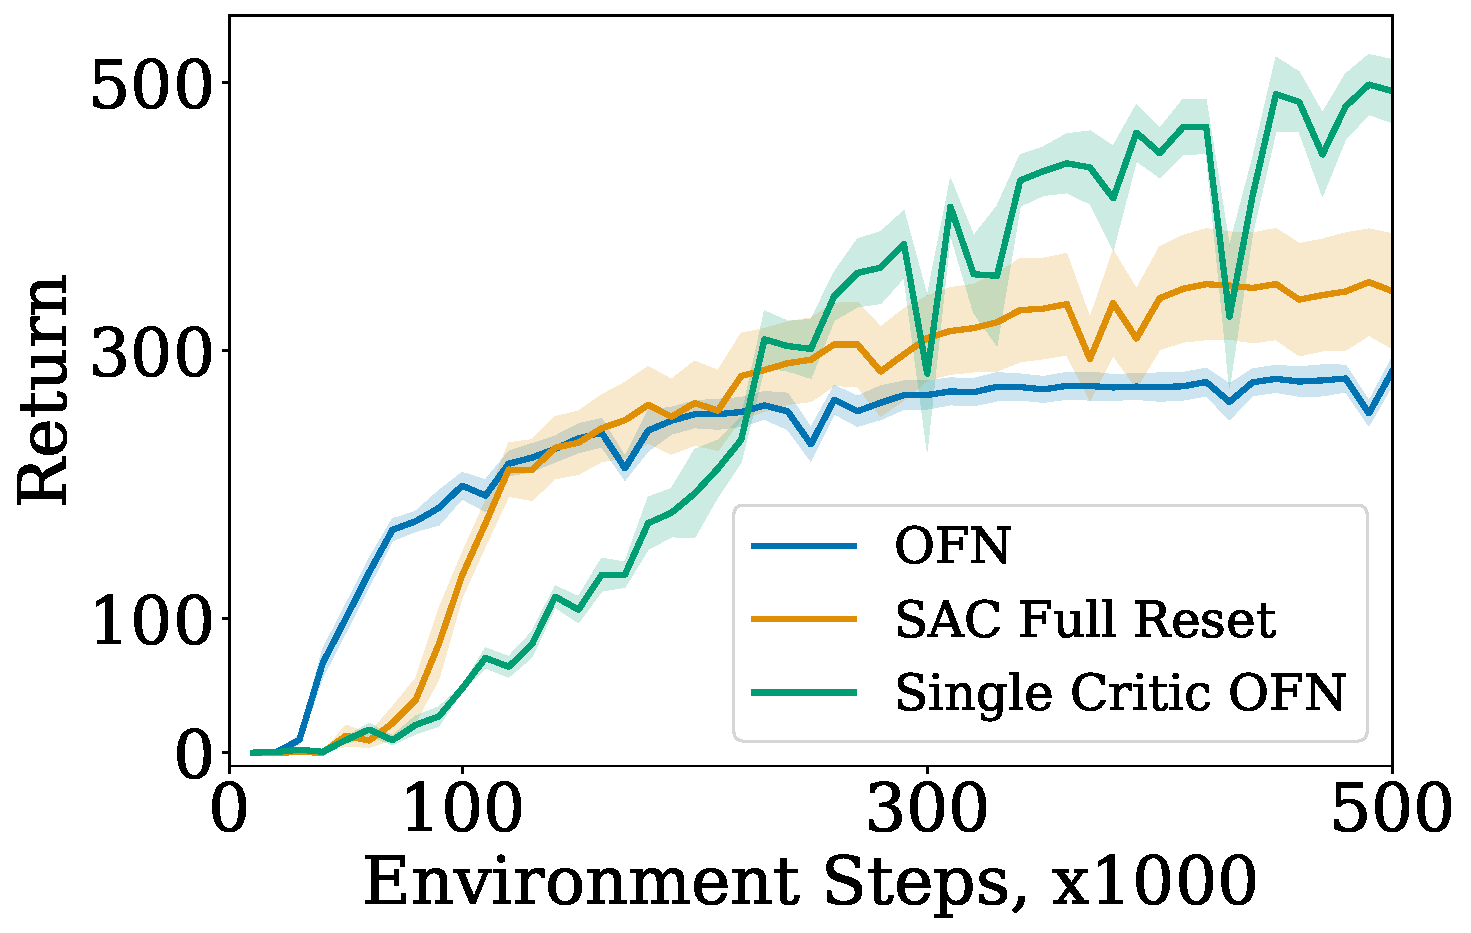
\includegraphics[width=4.25cm]{figures/dissecting/main_exp/hopper_hop_wl.pdf}
    \end{subfigure}%
    \caption{Mean return of single-critic OFN, standard OFN and resetting; $\mathrm{UTD}=32$ on hopper-hop. Shaded regions are standard error.}
    \label{fig:overestimationhopper_hop}
\end{minipage}
\end{figure}



To answer \textbf{Q1}, we compare OFN and SAC with resets on the DMC15-500k benchmark with large update ratios of $8$ and $32$ as proposed by \textcite{nikishin2022primacy} and  \textcite{schwarzer2023bigger}.  We report mean, interquartile mean (IQM) and median as well as $95\%$ bootstrapped confidence intervals aggregated over seeds and tasks,  following~\textcite{agarwal2021deep}. The results are shown in Figure~\ref{fig:overestimationaggregate}.

First, we observe that in both cases, $\mathrm{UTD}=8$ and $\mathrm{UTD}=32$, OFN can significantly improve over the non-resetting MLP baseline across all metrics. The value estimates that diverge seem to have been handeled properly (see Appendix~\ref{app:exp_q}); learning is maintained. We note that our approach with $\mathrm{UTD}=8$ achieves mean and IQM performance comparable to that of standard resetting with $\mathrm{UTD}=32$. In median and quantile performance, all $\mathrm{UTD}=32$ overlap, highlighting that outliers contribute to the performance measurement. Note that the overall performance drops slightly for the OFN-based approach when going from $\mathrm{UTD}=8$ to $\mathrm{UTD}=32$. We conjecture that there are other learning problems such as exploration that have not been treated by alleviating value divergence. However, these do not lead to complete failure to learn but rather slightly slower convergence. %

\subsection{Other failure modes: Exploration limitations} \label{sec:otherfailure}


To validate the hypothesis of other failures and answer \textbf{Q2}, we run two additional experiments. First, our current focus is on failures of the critic; our proposed mitigation does not address any further failures that might stem from the actor. We defer a more detailed analysis of actor failure cases to future work. Instead, we test the OFN-based architecture again and, for now, simply reset the actor to shed light on the existence of potential additional challenges.
For comparison, we also run a second experiment in which we reset all learned parameters, including the critic.

The results in Figure~\ref{fig:overestimationaggregate} indicate that actor resetting can account for a meaningful portion of OFN's performance decline when going from $\mathrm{UTD}=8$ to $\mathrm{UTD}=32$. The actor-reset results are within variance of the full-resetting standard MLP baseline. Further, we observe that there is still some additional benefit to resetting the critic as well. 
This does not invalidate the premise of our hypothesis, value divergence might not be the \emph{only} cause of problems in the high UTD case. We have provided significant evidence that it is a \emph{major} contributor.
Resetting both networks of OFN with $\mathrm{UTD}=32$  outperforms all other baselines on mean and IQM comparisons. %



To explain the remaining efficacy of critic resets, we examine the hopper-hop environment where standard SAC with resets outperforms OFN. 
In RL with function approximation, one might not only encounter over- but also under-estimation~\parencite{wu2020reducing, lan2020maxmin, saglam2021estimation}.
We believe that hopper  is sensitive to pessimism, and periodically resetting the networks might partially and temporarily counteract the inherent pessimism of the dual critic setup.

To obtain evidence for this conjecture, we repeated some experiments with a single critic. As OFN handles divergence it might not require a minimization over two critics~\parencite{fujimoto2018addressing}. We compare OFN using a single critic and $32$ updates per environment step to standard SAC and OFN in Figure~\ref{fig:overestimationhopper_hop}. With a single critic, OFN does not get stuck in a local minimum and outperforms full resetting. Note that this is only true in few environments, leading us to believe that the effects of high-update training are MDP-dependent.
In some environments we observe unstable learning with a single critic, which highlights that the bias countered by the double critic optimization and the overestimation from optimization we study are likely orthogonal phenomena that both need to be addressed.
Most likely, there is a difficult trade-off between optimization stability and encouraging sufficient exploration, which is an exciting avenue for future research.

\subsection{Limit-testing feature normalization}

\begin{figure}[t]
\centering
    \begin{subfigure}[b]{0.8\textwidth}
        \centering
        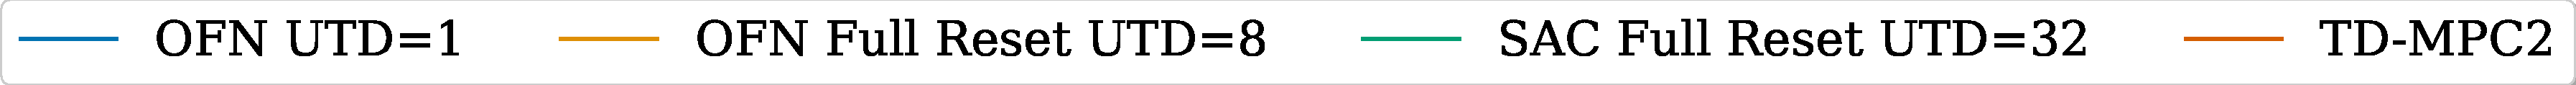
\includegraphics[height=0.4cm]{figures/dissecting/dog_exp/dog_legend.pdf}
    \end{subfigure}\\%
    \begin{subfigure}[t]{0.25\textwidth}
        \centering
        \label{subfig:overestimation:dog_stand}
    \end{subfigure}%
    \begin{subfigure}[t]{0.25\textwidth}
        \centering
        \label{subfig:overestimation:dog_walk}
    \end{subfigure}%
    \begin{subfigure}[t]{0.25\textwidth}
    \centering
        \label{subfig:overestimation:dog_trot}
    \end{subfigure}%
    \begin{subfigure}[t]{0.25\textwidth}
        \centering
        \label{subfig:overestimation:dog_run}
    \end{subfigure}%
    \caption{Mean return on the dog DMC tasks, comparing OFN to SAC with resets and the model-based TD-MPC2. Shaded regions indicate standard error. OFN outperforms SAC with resets, which is unable to learn and OFN with $\mathrm{UTD}=8$ and resetting is competitive with TD-MPC2.}
    \label{fig:overestimationall_dog}
\end{figure}

To answer \textbf{Q3}, we move to a set of training environments that is considered exceptionally hard for model-free approaches, namely the dog tasks of the DMC suite. Standard SAC can generally not obtain any reasonable reward and, due to their complex dynamics, these tasks are often tackled using model-based approaches such as TD-MPC2~\parencite{hansen2024tdmpc} with complicated update procedures and carefully tuned network architectures. We evaluate SAC and OFN on the dog tasks and compare against TD-MPC2 in Figure~\ref{fig:overestimationall_dog}.

First, observe that resetting without OFN obtains no improvement over a random policy. However, OFN with $\mathrm{UTD}=1$ can already obtain very good performance across all tasks, indicating that a major problem for SAC in these high-dimensional tasks is value divergence. When increasing the update ratio to $8$ and adding resetting, we improve the performance of the OFN agent even further and can match the reported results of the strong model-based TD-MPC2 baseline. 

We have already seen that resetting can take care of multiple optimization failures. However, these experiments also indicate that resetting is not a panacea as it is only effective when the initially learned policy can obtain some reward before being overwritten. 
This seems intuitive since resetting to a policy that cannot gather any useful data should not help. 
These results highlight that the early training dynamics of RL are highly important when it comes to training on complex environments and fitting early data correctly and quickly is crucial for success. 

This also opens up the question why resetting in the humanoid environments in the previous sections can yield success even though very little reward is observed. 
Besides greater divergence due to larger observation spaces in the dog MDPs, we suspect that this might be related to the complexity of exploration.
The ability of a random policy to obtain non-trivial reward and information about the environment has been shown to be a crucial factor in explaining the success of DRL methods in discrete environments~\parencite{laidlaw2023bridging}, and similar phenomena might be in effect here. 




\section{Related work}

Our work closely examines previous work on the primacy bias and the related resetting technique \parencite{anderson1992qlearning,nikishin2022primacy,doro2023barrier,schwarzer2023bigger}.
Going beyond, overestimation and feature learning challenges are a widely studied phenomenon in the literature.

{\bf Combatting overestimation}~~
Overestimation in off-policy value function learning is a well-established problem in the RL literature that dates back far before the prime times of deep learning~\parencite{thrun1993issues, precup2001off}. The effects of function approximation error and the effect on variance and bias have been studied~\parencite{pendrith1997estimator, mannor2007bias} as well.
With the rise of deep learning, researchers have tried to address the overestimation bias via algorithmic interventions such as combining multiple Q-learning predictors to achieve underestimation~\parencite{hasselt2010double, hasselt2016deep, zongzhang2017weighted, lan2020maxmin}, using averages over previous Q-values for variance reduction~\parencite{anschel2017averaged}, or general error term correction~\parencite{donghun2013bias, fox2016taming}. In the context of actor-critic methods, the twinned critic minimization approach of \textcite{fujimoto2018addressing} has become a de-facto standard. Most of these approaches are not applicable or break down under very high update ratios.
To regulate the overestimation-pessimism balance more carefully, several authors have attempted to use larger ensembles of independent Q-value estimates \parencite{lee2021sunrise,peer2021ensemble,chen2021randomized,hiraoka2022dropout}. Ensembling ideas were also combined with ideas from distributional RL~\parencite{bellemare2017distributional} to combat overestimation~\parencite{kuznetsov2020controlling}.  Instead of addressing the statistical bias in deep RL, our study focuses on the problems inherent to neural networks and gradient based optimization for value function estimation. Work from offline-to-online RL has demonstrated that standard layer normalization can bound value estimates during offline training and mitigate extrapolation while still allowing for exploration afterwards~\parencite{ball2023efficient}. Layer normalization has subsequently been used to achieve generally strong results in offline RL~\parencite{tarasov2023rebrac}. Our work is also related to a recent contribution using batch-normalization for increased computational efficiency by~\textcite{bhatt2024crossq} who focus on decreasing update ratios rather than increasing them. A concurrent work by~\textcite{nauman2024overestimation} provides a large scale study on different regularization techniques to combat overestimation. This work also demonstrates the efficacy of SAC on the dog tasks when properly regularized but it does not highlight the effects of Q-value divergence from exploding gradients as a key challenge for this set of environments.

{\bf Combating plasticity loss}~~ Another aspect of the primacy bias is the tendency of neural networks to lose their capacity for learning over time~\parencite{igl2021transient}, sometimes termed \emph{plasticity loss}~\parencite{lyle2022understanding, abbas2023loss}. Recent work mitigates plasticity loss using feature rank maximization~\parencite{kumar2021implicit}, regularization~\parencite{lyle2023understanding}, or learning a second copied network~\parencite{nikishin2024deep}. Some of the loss stems from neurons falling dormant over time~\parencite{sokar2023dormant}. A concurrent, closely related work by~\textcite{lyle2024disentangling} disentangles the causes for plasticity loss further. They use layer normalization to prevent some of these causes, which is closely related to our unit ball normalization. Our work differs in that we focus on the setting of high update ratios and use stronger constraints to mitigate value divergence rather than plasticity loss. 


\section{Conclusion}

By dissecting the effects underlying the primacy bias, we have identified a crucial challenge: \emph{value divergence}. 
While the main focus in studying increased Q-value has been on the statistical bias inherent in off-policy sampling, we show that Q-value divergence can arise due to problems inherent to neural network optimization.
This optimization-caused divergence can be mitigated using the unit-ball normalization approach, which shines on the \textsf{dm\_control} benchmark with its simplicity and efficacy. 
With this result, we challenge the assumption that failure to learn in high-UTD settings primarily stems from \emph{overfitting} early data by showing that combating value divergence is competitive with resetting networks. 
This offers a starting point towards explaining the challenges of high-UTD training in more detail and opens the path towards even more performant and sample efficient RL in the future.

This chapter shines a light on the important role that the implicit representations learned from end-to-end critic optimization play in value function learning.
In essence, model-free value learning is a purely \emph{decision-aware} method, as it solely focuses on extracting good features for the current value prediction target.
But due to the deep entanglement between optimization, exploration, and non-stationary data, we can see that relying solely on end-to-end learning for value estimation is a potentially perilous endeavour.
While simple regularization can already alleviate some of the issues with value learning,  the next chapter takes an in-depth look at more explicit ways of constructing good representative features.
